\section{Conclusions}\label{sec:conclusions}

The methods presented above are implemented in the Python package \texttt{Bayesian\_pyhf}~\cite{BayesianPyhf}. This software package enables the parallel Bayesian and frequentist analysis of multi-channel binned models within the single software framework \texttt{pyhf}.\\
The current interface of the package \texttt{Bayesian\_pyhf} is demonstrated in Fig.~\ref{code}.
    \begin{figure} %[H]
        \centering
        % \captionsetup{justification=centering}
        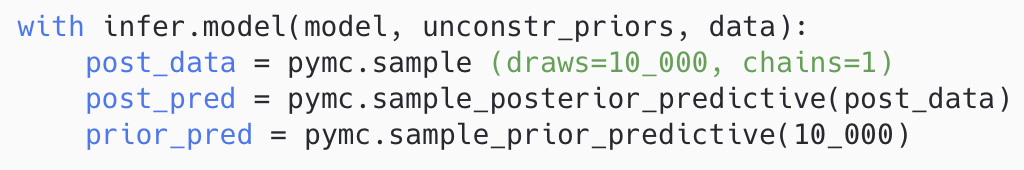
\includegraphics[width=9cm]{figures/code2.png}
        \centering
        \caption{Pseudo-code for evaluating \texttt{HistFactory} models (\texttt{model}) using \texttt{PyMC} given unconstrained parameters (\texttt{unconstr\_priors}) and observations (\texttt{data}). \texttt{post(prior)\_pred} are the posterior (prior) predictives and \texttt{post\_data} are the samples from the posterior distribution. Following the \texttt{PyMC} syntax~\cite{PyMC}, the \texttt{with} statement opens a context, that initializes the inference in a way that all actions within the block are interpreted with respect to the given model, data and priors. In addition, the methodologies regarding conjugate priors from Sec.~\ref{subsec:HFandpyhf} are applied under the hood, resulting in the constraint priors which are added to the model parameters for sampling.}
        \label{code}
    \end{figure}
\noindent Further enhancements regarding the user interface and stability with respect to multi-chain sampling are ongoing. A full integration in the \texttt{pyhf} library is also planned.
